%!TEX TS-program = xelatex
%!TEX encoding = UTF-8 Unicode
% Awesome CV LaTeX Template for CV/Resume
%
% This template has been downloaded from:
% https://github.com/posquit0/Awesome-CV
%
% Author:
% Claud D. Park <posquit0.bj@gmail.com>
% http://www.posquit0.com
%
% Template license:
% CC BY-SA 4.0 (https://creativecommons.org/licenses/by-sa/4.0/)
%


%-------------------------------------------------------------------------------
% CONFIGURATIONS
%-------------------------------------------------------------------------------
% A4 paper size by default, use 'letterpaper' for US letter
\documentclass[11pt, a4paper]{awesome-cv}

% Configure page margins with geometry
\geometry{left=1.4cm, top=.8cm, right=1.4cm, bottom=1.8cm, footskip=.5cm}

% Specify the location of the included fonts
\fontdir[fonts/]

% Color for highlights
% Awesome Colors: awesome-emerald, awesome-skyblue, awesome-red, awesome-pink, awesome-orange
%                 awesome-nephritis, awesome-concrete, awesome-darknight
\colorlet{awesome}{awesome-red}
% Uncomment if you would like to specify your own color
% \definecolor{awesome}{HTML}{CA63A8}

% Colors for text
% Uncomment if you would like to specify your own color
% \definecolor{darktext}{HTML}{414141}
% \definecolor{text}{HTML}{333333}
% \definecolor{graytext}{HTML}{5D5D5D}
% \definecolor{lighttext}{HTML}{999999}

% Set false if you don't want to highlight section with awesome color
\setbool{acvSectionColorHighlight}{false}

% If you would like to change the social information separator from a pipe (|) to something else
\renewcommand{\acvHeaderSocialSep}{\quad\textbar\quad}

% Define an environment for cvpub
\newenvironment{cvpubs}{%
  \vspace{\acvSectionContentTopSkip}
    \vspace{-2mm}
    \paragraphstyle
}{%
    \par
    \vspace{1mm}
}

% Define a line of cvpub
% Usage: \cvpub{<ciation>}

\newcommand{\field}[1]{\textbf{#1}}
\usepackage{graphicx}
\usepackage{adjustbox}
\usepackage{xeCJK}
\usepackage{xstring}
% CHINESE_COMPANY CHINESE_UNIVERSITY ENGLISH 
%\newcommand{\COMPILEMODE}{ENGLISH}
%\newcommand{\COMPILEMODE}{CHINESE_COMPANY}
\newcommand{\COMPILEMODE}{CHINESE_UNIVERSITY}
%{Songti SC}
\setCJKmainfont[Path=/System/Library/Fonts/Supplemental/]{Songti.ttc}

%-------------------------------------------------------------------------------
%	PERSONAL INFORMATION
%	Comment any of the lines below if they are not required
%-------------------------------------------------------------------------------
% Available options: circle|rectangle,edge/noedge,left/right
% \photo{./examples/profile.png}
\IfStrEq{\COMPILEMODE}{ENGLISH}{
	\name{RESUME}{}
}{
	\name{简历}{}
}

%\position{Software Architect{\enskip\cdotp\enskip}Security Expert}
%\address{42-8, Bangbae-ro 15-gil, Seocho-gu, Seoul, 00681, Rep. of KOREA}

%\mobile{(+82) 10-9030-1843}
%\email{posquit0.bj@gmail.com}
%\dateofbirth{January 1st, 1970}
%\homepage{www.posquit0.com}
%\github{posquit0}
%\linkedin{posquit0}
% \gitlab{gitlab-id}
% \stackoverflow{SO-id}{SO-name}
% \twitter{@twit}
% \skype{skype-id}
% \reddit{reddit-id}
% \medium{medium-id}
% \kaggle{kaggle-id}
% \googlescholar{googlescholar-id}{name-to-display}
%% \firstname and \lastname will be used
% \googlescholar{googlescholar-id}{}
% \extrainfo{extra information}

%\quote{``Be the change that you want to see in the world."}


%-------------------------------------------------------------------------------
\begin{document}

% Print the header with above personal information
% Give optional argument to change alignment(C: center, L: left, R: right)
\makecvheader

% Print the footer with 3 arguments(<left>, <center>, <right>)
% Leave any of these blank if they are not needed


%-------------------------------------------------------------------------------
%	CV/RESUME CONTENT
%	Each section is imported separately, open each file in turn to modify content
%-------------------------------------------------------------------------------
\IfStrEq{\COMPILEMODE}{CHINESE_COMPANY}{
	\cvsection{基本情况}

\begin{minipage}{0.2\textwidth}
	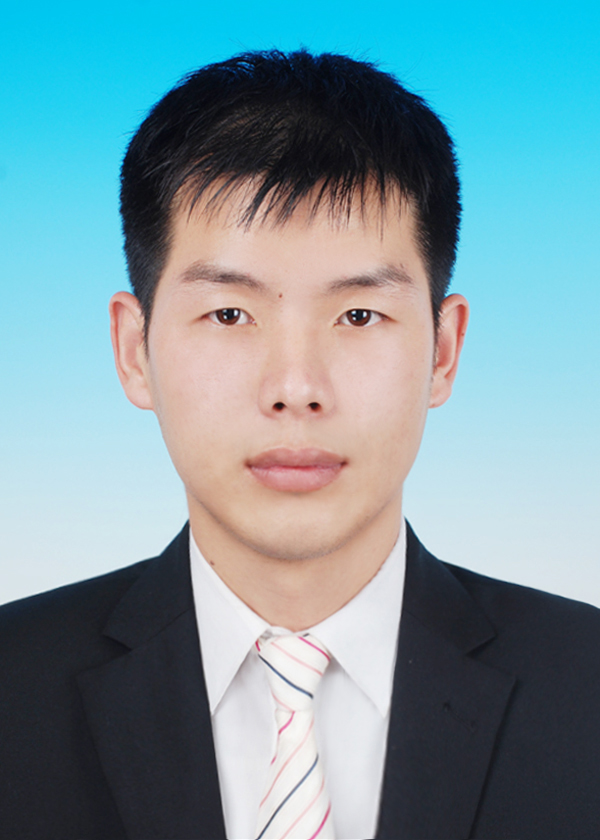
\includegraphics[scale=1.1]{8574.png}
\end{minipage}
\hfill
\begin{minipage}{0.8\textwidth}
	\renewcommand{\arraystretch}{2.2}
	\begin{adjustbox}{width=1\linewidth}
		\begin{tabular}{lcr}
			姓名: 张辉耀 & 性别:男 & 出生年月:1991.01.10 \\
			学历学位:博士研究生 & 政治面貌: 中共党员 & 婚否:未婚 \\
			邮箱: zhanghuiyao2357@163.com & 联系电话:152-1679-7320 & 户口所在地:河南驻马店 \\
			个人网站:\url{https://slip-slap.github.io/} & & 
		\end{tabular}
	\renewcommand{\arraystretch}{0.5}
	\end{adjustbox}
\end{minipage}




	\makecvfooter
	  {\today}
	  {张辉耀~~~·~~~简历}
	  {\thepage}
	%-------------------------------------------------------------------------------
%	SECTION TITLE
%-------------------------------------------------------------------------------
\cvsection{}


%-------------------------------------------------------------------------------
%	CONTENT
%-------------------------------------------------------------------------------
\begin{cvparagraph}
研究生时期的导师为我打开了计算机世界的大门,从此以后,编程和数学从兴趣变成热爱。在过去六年的学术生涯中,
致力于研究先进的模型,算法在纺织服装,材料领域的应用和实践,并在计算机类的学术期刊上发表有两篇学术论文。使用的编程语言也从Matlab,到Java,到现在的python,C++。
为了方便学习和记录,把近些年的学习笔记放到个人GitHub网站上。未来主要想从事机器学习,数据科学以及人工智能方向的研究工作。
\end{cvparagraph}

	%-------------------------------------------------------------------------------
%	SECTION TITLE
%-------------------------------------------------------------------------------
\cvsection{Education}


%-------------------------------------------------------------------------------
%	CONTENT
%-------------------------------------------------------------------------------
\begin{cventries}

%---------------------------------------------------------
  \cventry
    {B.S. in Computer Science and Engineering} % Degree
    {POSTECH(Pohang University of Science and Technology)} % Institution
    {Pohang, S.Korea} % Location
    {Mar. 2010 - Aug. 2017} % Date(s)
    {
      \begin{cvitems} % Description(s) bullet points
        \item {Got a Chun Shin-Il Scholarship which is given to promising students in CSE Dept.}
      \end{cvitems}
    }

%---------------------------------------------------------
\end{cventries}

	%-------------------------------------------------------------------------------
%	SECTION TITLE
%-------------------------------------------------------------------------------
\cvsection{Research}

%-------------------------------------------------------------------------------
%	CONTENT
%-------------------------------------------------------------------------------
\begin{cventries}

%---------------------------------------------------------
  \cventry
    {Professor: Yokoyama Atsushi} % Advisor
    {Kyoto Institute of Technology} % Institution
    {Japan, Kyoto} % Location
    {2018.9 - now} % Date(s)
    {
      \begin{cvitems} % Description(s)
%		\item { The multiple constrained optimization based on a variant of
%				genetic algorithm(GA). GA is an efficient and robust algorithm
%				to solve the optimization problem in terms of discrete
%				variables.  However, intially GA was proposed for unconstrained
%				problem, to solve constrained problem, we have to reformulate
%				the objective function, in which append the constraints to the
%%				objective function as punishment items. To overcome the
 %   			inherient drawback, we propose a new genetic algorithm with two
 %   			techniques: mating pool classification and self-adaptive
 %   			mutaiton.  Then we adopt this new genetic algorithm to guide the
 %   			design of a laminate under single or multiple constraints.}
 %   			
 %%   	\item { The topology design of an artifical neural network(ANN) based on
  %  			genetic algorithm. Artifical neural networks are widely used for
  %  			various scenarios, such as prediction, classification,
  %  			optimization, in which the topology of an ANN plays a critical
  %  			role of the performance. We propose a three-layer ANN model, in
  %  			which the design variables are the number of neurons in the
  %%  			hidden layer, the active function, and the connection
   % 			relationship. Genetic algorithm is adopted to guide the search
   % 			process, and the one with best performance is used to predict
   % 			the strength of angle ply laminate. The advantage of the method
   % 			is to reduce the computaiton cost and simplify the
   % 			calculation process, compared with the tradional complicated
   % 			mathematical model.}
    %  \end{cvitems}
    }

%---------------------------------------------------------
  \cventry
    {Professor: Yueqi Zhong} % Advisor
    {Donghua University} % Institution
    {China, Shanghai} % Location
    {2015.9-2018.3} % Date(s)
    {
      \begin{cvitems} % Description(s)
        \item
			{
				The separation of connected curve based on convex hull algorithm
				and the elliptic curve fitting based on fourier transforamtion. 
				Convex hull algorithm is used to obtain the smallest convex
				polygon which encloses a set of points. Fourier transforamtion
				can be used to remove noises on a curve. The human body data
				points can be obtained through a three-dimensional scan device, 
				and the shape of transverse section of human body depends on the
				the cutting point. For the transverse section at the armpit, the
				shape of the cross section is a joint curve of three circles. We
				can use convex hull algorithm to find the separtion point. For
				the cross section at the waist, the corresponding shape is a
				circle with noises, and fourier transforamtion can remove the
				noise on the curve.
			}
      \end{cvitems}
    }

%---------------------------------------------------------
\end{cventries}

	%-------------------------------------------------------------------------------
%	SECTION TITLE
%-------------------------------------------------------------------------------
\cvsection{Publications}


%-------------------------------------------------------------------------------
%	CONTENT
%-------------------------------------------------------------------------------

%---------------------------------------------------------
%\cvsubsection{}
%---------------------------------------------------------


\begin{cvpubs}

%	\cvpub{
	\textbf{Huiyao Zhang}, Atsushi Yokoyama. 2022. Optimum Design of
	Laminated Composites for Minimum Thickness by a Variant of Genetic
Algorithm. Journal of Textile Engineering(accepted). 
%[收录: Scopus]
%}
	
%	\cvpub{
		\textbf{Huiyao Zhang}, Atsushi Yokoyama. 2021. A Technique for
		Constrained Optimization of Cross-ply Laminates Using a New Variant of
	Genetic Algorithm. International Journal of Advanced Computer Science and Applications, 12(6): 760-767. 
%[收录: Scopus/Web of Science(ESCI), 影响因子: 1.09]
%}

%	\cvpub{
		\textbf{Huiyao Zhang}, Atsushi Yokoyama. 2021. Predicting Strength
	Ratio of Laminated Composite Material with Evolutionary Artificial Neural
	Network. International Journal of Advanced Computer Science and Applications,
12(6): 11-18. 
%[收录: Scopus/Web of Science(ESCI),影响因子: 1.09]
%}

	%\cvpub{
		\textbf{Hui-Yao Zhang}, Duan Li, Hao-Yang Xie, Yue-Qi Zhong. 2017.
	A Study on the Female Chest Contour with Elliptic Fourier Analysis.
Journal of Fiber Bioengineering and Informatics, 10(3): 131-139.  %}

	%\cvpub{
		\textbf{Hui-Yao Zhang}, Duan Li, Hao-Yang Xie, Yue-Qi Zhong. 2017.
	Elliptic Fourier Analysis on Female Chest Contour. Textile Bioengineering
		and Informatics Symposium. 
%	[收录: CPCI(ISTP)/Scopus/Ei Compendex ]
	%}
\end{cvpubs}

% %---------------------------------------------------------
%\cvsubsection{In Review}
% %---------------------------------------------------------

%\begin{cvpubs}
%    \cvpub{Manuscript 1}

%    \cvpub{Manuscript 2}
%\end{cvpubs}

% %---------------------------------------------------------
%\cvsubsection{In Prep}
% %---------------------------------------------------------

%\begin{cvpubs}
%\small \color{black}
%    \cvpub{Manuscript 1}

%    \cvpub{Manuscript 2}
%\end{cvpubs}

% %---------------------------------------------------------

	%-------------------------------------------------------------------------------
%	SECTION TITLE
%-------------------------------------------------------------------------------
\cvsection{Presentation}


%-------------------------------------------------------------------------------
%	CONTENT
%-------------------------------------------------------------------------------
\begin{cventries}

%---------------------------------------------------------
  \cventry
    {Presenter for <Hosting Web Application for Free utilizing GitHub, Netlify and CloudFlare>} % Role
    {DevFest Seoul by Google Developer Group Korea} % Event
    {Seoul, S.Korea} % Location
    {Nov. 2017} % Date(s)
    {
      \begin{cvitems} % Description(s)
        \item {Introduced the history of web technology and the JAM stack which is for the modern web application development.}
        \item {Introduced how to freely host the web application with high performance utilizing global CDN services.}
      \end{cvitems}
    }

%---------------------------------------------------------
  \cventry
    {Presenter for <DEFCON 20th : The way to go to Las Vegas>} % Role
    {6th CodeEngn (Reverse Engineering Conference)} % Event
    {Seoul, S.Korea} % Location
    {Jul. 2012} % Date(s)
    {
      \begin{cvitems} % Description(s)
        \item {Introduced CTF(Capture the Flag) hacking competition and advanced techniques and strategy for CTF}
      \end{cvitems}
    }

%---------------------------------------------------------
  \cventry
    {Presenter for <Metasploit 101>} % Role
    {6th Hacking Camp - S.Korea} % Event
    {S.Korea} % Location
    {Sep. 2012} % Date(s)
    {
      \begin{cvitems} % Description(s)
        \item {Introduced basic procedure for penetration testing and how to use Metasploit}
      \end{cvitems}
    }

%---------------------------------------------------------
\end{cventries}

	%-------------------------------------------------------------------------------
%	SECTION TITLE
%-------------------------------------------------------------------------------
\cvsection{Skills}


%-------------------------------------------------------------------------------
%	CONTENT
%-------------------------------------------------------------------------------
\begin{cvskills}

%---------------------------------------------------------
  \cvskill
    {DevOps} % Category
    {AWS, Docker, Kubernetes, Rancher, Vagrant, Packer, Terraform, Jenkins, CircleCI} % Skills

%---------------------------------------------------------
  \cvskill
    {Back-end} % Category
    {Koa, Express, Django, REST API} % Skills

%---------------------------------------------------------
  \cvskill
    {Front-end} % Category
    {Hugo, Redux, React, HTML5, LESS, SASS} % Skills

%---------------------------------------------------------
  \cvskill
    {Programming} % Category
    {Node.js, Python, JAVA, OCaml, LaTeX} % Skills

%---------------------------------------------------------
  \cvskill
    {Languages} % Category
    {Korean, English, Japanese} % Skills

%---------------------------------------------------------
\end{cvskills}

	%-------------------------------------------------------------------------------
%	SECTION TITLE
%-------------------------------------------------------------------------------
\cvsection{Honors \& Awards}


%-------------------------------------------------------------------------------
%	SUBSECTION TITLE
%-------------------------------------------------------------------------------
\cvsubsection{International}


%-------------------------------------------------------------------------------
%	CONTENT
%-------------------------------------------------------------------------------
\begin{cvhonors}

%---------------------------------------------------------
  \cvhonor
    {Finalist} % Award
    {DEFCON 26th CTF Hacking Competition World Final} % Event
    {Las Vegas, U.S.A} % Location
    {2018} % Date(s)

%---------------------------------------------------------
  \cvhonor
    {Finalist} % Award
    {DEFCON 25th CTF Hacking Competition World Final} % Event
    {Las Vegas, U.S.A} % Location
    {2017} % Date(s)

%---------------------------------------------------------
  \cvhonor
    {Finalist} % Award
    {DEFCON 22nd CTF Hacking Competition World Final} % Event
    {Las Vegas, U.S.A} % Location
    {2014} % Date(s)

%---------------------------------------------------------
  \cvhonor
    {Finalist} % Award
    {DEFCON 21st CTF Hacking Competition World Final} % Event
    {Las Vegas, U.S.A} % Location
    {2013} % Date(s)

%---------------------------------------------------------
  \cvhonor
    {Finalist} % Award
    {DEFCON 19th CTF Hacking Competition World Final} % Event
    {Las Vegas, U.S.A} % Location
    {2011} % Date(s)

%---------------------------------------------------------
  \cvhonor
    {6th Place} % Award
    {SECUINSIDE Hacking Competition World Final} % Event
    {Seoul, S.Korea} % Location
    {2012} % Date(s)

%---------------------------------------------------------
\end{cvhonors}


%-------------------------------------------------------------------------------
%	SUBSECTION TITLE
%-------------------------------------------------------------------------------
\cvsubsection{Domestic}


%-------------------------------------------------------------------------------
%	CONTENT
%-------------------------------------------------------------------------------
\begin{cvhonors}

%---------------------------------------------------------
  \cvhonor
    {3rd Place} % Award
    {WITHCON Hacking Competition Final} % Event
    {Seoul, S.Korea} % Location
    {2015} % Date(s)

%---------------------------------------------------------
  \cvhonor
    {Silver Prize} % Award
    {KISA HDCON Hacking Competition Final} % Event
    {Seoul, S.Korea} % Location
    {2017} % Date(s)

%---------------------------------------------------------
  \cvhonor
    {Silver Prize} % Award
    {KISA HDCON Hacking Competition Final} % Event
    {Seoul, S.Korea} % Location
    {2013} % Date(s)

%---------------------------------------------------------
  \cvhonor
    {2nd Award} % Award
    {HUST Hacking Festival} % Event
    {S.Korea} % Location
    {2013} % Date(s)

%---------------------------------------------------------
  \cvhonor
    {3rd Award} % Award
    {HUST Hacking Festival} % Event
    {S.Korea} % Location
    {2010} % Date(s)

%---------------------------------------------------------
  \cvhonor
    {3rd Award} % Award
    {Holyshield 3rd Hacking Festival} % Event
    {S.Korea} % Location
    {2012} % Date(s)

%---------------------------------------------------------
  \cvhonor
    {2nd Award} % Award
    {Holyshield 3rd Hacking Festival} % Event
    {S.Korea} % Location
    {2011} % Date(s)

%---------------------------------------------------------
  \cvhonor
    {5th Place} % Award
    {PADOCON Hacking Competition Final} % Event
    {Seoul, S.Korea} % Location
    {2011} % Date(s)

%---------------------------------------------------------
\end{cvhonors}

}

\IfStrEq{\COMPILEMODE}{CHINESE_UNIVERSITY}{
	\cvsection{基本情况}

\begin{minipage}{0.2\textwidth}
	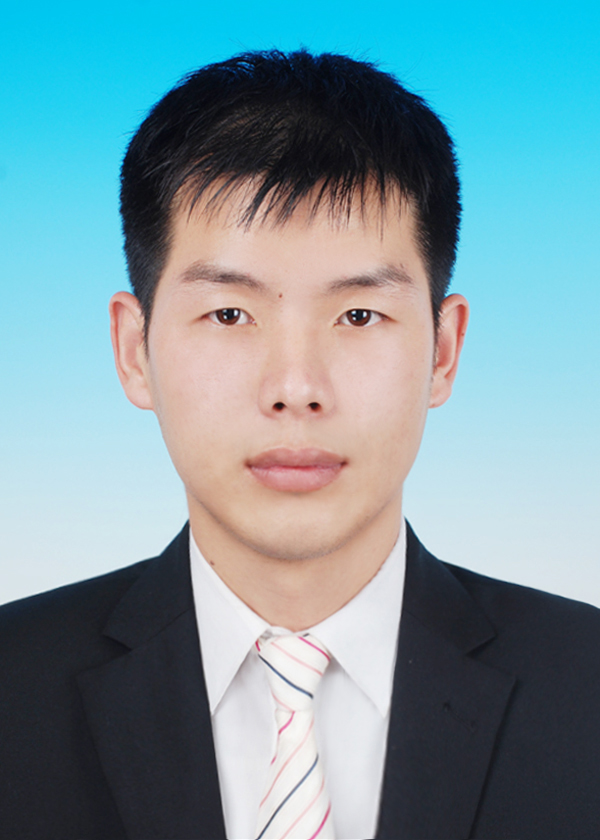
\includegraphics[scale=1.1]{8574.png}
\end{minipage}
\hfill
\begin{minipage}{0.8\textwidth}
	\renewcommand{\arraystretch}{2.2}
	\begin{adjustbox}{width=1\linewidth}
		\begin{tabular}{lcr}
			姓名: 张辉耀 & 性别:男 & 出生年月:1991.01.10 \\
			学历学位:博士研究生 & 政治面貌: 中共党员 & 婚否:未婚 \\
			邮箱: zhanghuiyao2357@163.com & 联系电话:152-1679-7320 & 户口所在地:河南驻马店 \\
			个人网站:\url{https://slip-slap.github.io/} & & 
		\end{tabular}
	\renewcommand{\arraystretch}{0.5}
	\end{adjustbox}
\end{minipage}




	\makecvfooter
	  {\today}
	  {张辉耀~~~·~~~简历}
	  {\thepage}
	%-------------------------------------------------------------------------------
%	SECTION TITLE
%-------------------------------------------------------------------------------
\cvsection{}


%-------------------------------------------------------------------------------
%	CONTENT
%-------------------------------------------------------------------------------
\begin{cvparagraph}
研究生时期的导师为我打开了计算机世界的大门,从此以后,编程和数学从兴趣变成热爱。在过去六年的学术生涯中,
致力于研究先进的模型,算法在纺织服装,材料领域的应用和实践,并在计算机类的学术期刊上发表有两篇学术论文。使用的编程语言也从Matlab,到Java,到现在的python,C++。
为了方便学习和记录,把近些年的学习笔记放到个人GitHub网站上。未来主要想从事机器学习,数据科学以及人工智能方向的研究工作。
\end{cvparagraph}

	%-------------------------------------------------------------------------------
%	SECTION TITLE
%-------------------------------------------------------------------------------
\cvsection{Education}


%-------------------------------------------------------------------------------
%	CONTENT
%-------------------------------------------------------------------------------
\begin{cventries}

%---------------------------------------------------------
  \cventry
    {B.S. in Computer Science and Engineering} % Degree
    {POSTECH(Pohang University of Science and Technology)} % Institution
    {Pohang, S.Korea} % Location
    {Mar. 2010 - Aug. 2017} % Date(s)
    {
      \begin{cvitems} % Description(s) bullet points
        \item {Got a Chun Shin-Il Scholarship which is given to promising students in CSE Dept.}
      \end{cvitems}
    }

%---------------------------------------------------------
\end{cventries}

	%-------------------------------------------------------------------------------
%	SECTION TITLE
%-------------------------------------------------------------------------------
\cvsection{Research}

%-------------------------------------------------------------------------------
%	CONTENT
%-------------------------------------------------------------------------------
\begin{cventries}

%---------------------------------------------------------
  \cventry
    {Professor: Yokoyama Atsushi} % Advisor
    {Kyoto Institute of Technology} % Institution
    {Japan, Kyoto} % Location
    {2018.9 - now} % Date(s)
    {
      \begin{cvitems} % Description(s)
%		\item { The multiple constrained optimization based on a variant of
%				genetic algorithm(GA). GA is an efficient and robust algorithm
%				to solve the optimization problem in terms of discrete
%				variables.  However, intially GA was proposed for unconstrained
%				problem, to solve constrained problem, we have to reformulate
%				the objective function, in which append the constraints to the
%%				objective function as punishment items. To overcome the
 %   			inherient drawback, we propose a new genetic algorithm with two
 %   			techniques: mating pool classification and self-adaptive
 %   			mutaiton.  Then we adopt this new genetic algorithm to guide the
 %   			design of a laminate under single or multiple constraints.}
 %   			
 %%   	\item { The topology design of an artifical neural network(ANN) based on
  %  			genetic algorithm. Artifical neural networks are widely used for
  %  			various scenarios, such as prediction, classification,
  %  			optimization, in which the topology of an ANN plays a critical
  %  			role of the performance. We propose a three-layer ANN model, in
  %  			which the design variables are the number of neurons in the
  %%  			hidden layer, the active function, and the connection
   % 			relationship. Genetic algorithm is adopted to guide the search
   % 			process, and the one with best performance is used to predict
   % 			the strength of angle ply laminate. The advantage of the method
   % 			is to reduce the computaiton cost and simplify the
   % 			calculation process, compared with the tradional complicated
   % 			mathematical model.}
    %  \end{cvitems}
    }

%---------------------------------------------------------
  \cventry
    {Professor: Yueqi Zhong} % Advisor
    {Donghua University} % Institution
    {China, Shanghai} % Location
    {2015.9-2018.3} % Date(s)
    {
      \begin{cvitems} % Description(s)
        \item
			{
				The separation of connected curve based on convex hull algorithm
				and the elliptic curve fitting based on fourier transforamtion. 
				Convex hull algorithm is used to obtain the smallest convex
				polygon which encloses a set of points. Fourier transforamtion
				can be used to remove noises on a curve. The human body data
				points can be obtained through a three-dimensional scan device, 
				and the shape of transverse section of human body depends on the
				the cutting point. For the transverse section at the armpit, the
				shape of the cross section is a joint curve of three circles. We
				can use convex hull algorithm to find the separtion point. For
				the cross section at the waist, the corresponding shape is a
				circle with noises, and fourier transforamtion can remove the
				noise on the curve.
			}
      \end{cvitems}
    }

%---------------------------------------------------------
\end{cventries}

	%-------------------------------------------------------------------------------
%	SECTION TITLE
%-------------------------------------------------------------------------------
\cvsection{Publications}


%-------------------------------------------------------------------------------
%	CONTENT
%-------------------------------------------------------------------------------

%---------------------------------------------------------
%\cvsubsection{}
%---------------------------------------------------------


\begin{cvpubs}

%	\cvpub{
	\textbf{Huiyao Zhang}, Atsushi Yokoyama. 2022. Optimum Design of
	Laminated Composites for Minimum Thickness by a Variant of Genetic
Algorithm. Journal of Textile Engineering(accepted). 
%[收录: Scopus]
%}
	
%	\cvpub{
		\textbf{Huiyao Zhang}, Atsushi Yokoyama. 2021. A Technique for
		Constrained Optimization of Cross-ply Laminates Using a New Variant of
	Genetic Algorithm. International Journal of Advanced Computer Science and Applications, 12(6): 760-767. 
%[收录: Scopus/Web of Science(ESCI), 影响因子: 1.09]
%}

%	\cvpub{
		\textbf{Huiyao Zhang}, Atsushi Yokoyama. 2021. Predicting Strength
	Ratio of Laminated Composite Material with Evolutionary Artificial Neural
	Network. International Journal of Advanced Computer Science and Applications,
12(6): 11-18. 
%[收录: Scopus/Web of Science(ESCI),影响因子: 1.09]
%}

	%\cvpub{
		\textbf{Hui-Yao Zhang}, Duan Li, Hao-Yang Xie, Yue-Qi Zhong. 2017.
	A Study on the Female Chest Contour with Elliptic Fourier Analysis.
Journal of Fiber Bioengineering and Informatics, 10(3): 131-139.  %}

	%\cvpub{
		\textbf{Hui-Yao Zhang}, Duan Li, Hao-Yang Xie, Yue-Qi Zhong. 2017.
	Elliptic Fourier Analysis on Female Chest Contour. Textile Bioengineering
		and Informatics Symposium. 
%	[收录: CPCI(ISTP)/Scopus/Ei Compendex ]
	%}
\end{cvpubs}

% %---------------------------------------------------------
%\cvsubsection{In Review}
% %---------------------------------------------------------

%\begin{cvpubs}
%    \cvpub{Manuscript 1}

%    \cvpub{Manuscript 2}
%\end{cvpubs}

% %---------------------------------------------------------
%\cvsubsection{In Prep}
% %---------------------------------------------------------

%\begin{cvpubs}
%\small \color{black}
%    \cvpub{Manuscript 1}

%    \cvpub{Manuscript 2}
%\end{cvpubs}

% %---------------------------------------------------------

	%-------------------------------------------------------------------------------
%	SECTION TITLE
%-------------------------------------------------------------------------------
\cvsection{Presentation}


%-------------------------------------------------------------------------------
%	CONTENT
%-------------------------------------------------------------------------------
\begin{cventries}

%---------------------------------------------------------
  \cventry
    {Presenter for <Hosting Web Application for Free utilizing GitHub, Netlify and CloudFlare>} % Role
    {DevFest Seoul by Google Developer Group Korea} % Event
    {Seoul, S.Korea} % Location
    {Nov. 2017} % Date(s)
    {
      \begin{cvitems} % Description(s)
        \item {Introduced the history of web technology and the JAM stack which is for the modern web application development.}
        \item {Introduced how to freely host the web application with high performance utilizing global CDN services.}
      \end{cvitems}
    }

%---------------------------------------------------------
  \cventry
    {Presenter for <DEFCON 20th : The way to go to Las Vegas>} % Role
    {6th CodeEngn (Reverse Engineering Conference)} % Event
    {Seoul, S.Korea} % Location
    {Jul. 2012} % Date(s)
    {
      \begin{cvitems} % Description(s)
        \item {Introduced CTF(Capture the Flag) hacking competition and advanced techniques and strategy for CTF}
      \end{cvitems}
    }

%---------------------------------------------------------
  \cventry
    {Presenter for <Metasploit 101>} % Role
    {6th Hacking Camp - S.Korea} % Event
    {S.Korea} % Location
    {Sep. 2012} % Date(s)
    {
      \begin{cvitems} % Description(s)
        \item {Introduced basic procedure for penetration testing and how to use Metasploit}
      \end{cvitems}
    }

%---------------------------------------------------------
\end{cventries}

	%-------------------------------------------------------------------------------
%	SECTION TITLE
%-------------------------------------------------------------------------------
\cvsection{Skills}


%-------------------------------------------------------------------------------
%	CONTENT
%-------------------------------------------------------------------------------
\begin{cvskills}

%---------------------------------------------------------
  \cvskill
    {DevOps} % Category
    {AWS, Docker, Kubernetes, Rancher, Vagrant, Packer, Terraform, Jenkins, CircleCI} % Skills

%---------------------------------------------------------
  \cvskill
    {Back-end} % Category
    {Koa, Express, Django, REST API} % Skills

%---------------------------------------------------------
  \cvskill
    {Front-end} % Category
    {Hugo, Redux, React, HTML5, LESS, SASS} % Skills

%---------------------------------------------------------
  \cvskill
    {Programming} % Category
    {Node.js, Python, JAVA, OCaml, LaTeX} % Skills

%---------------------------------------------------------
  \cvskill
    {Languages} % Category
    {Korean, English, Japanese} % Skills

%---------------------------------------------------------
\end{cvskills}

	%-------------------------------------------------------------------------------
%	SECTION TITLE
%-------------------------------------------------------------------------------
\cvsection{Honors \& Awards}


%-------------------------------------------------------------------------------
%	SUBSECTION TITLE
%-------------------------------------------------------------------------------
\cvsubsection{International}


%-------------------------------------------------------------------------------
%	CONTENT
%-------------------------------------------------------------------------------
\begin{cvhonors}

%---------------------------------------------------------
  \cvhonor
    {Finalist} % Award
    {DEFCON 26th CTF Hacking Competition World Final} % Event
    {Las Vegas, U.S.A} % Location
    {2018} % Date(s)

%---------------------------------------------------------
  \cvhonor
    {Finalist} % Award
    {DEFCON 25th CTF Hacking Competition World Final} % Event
    {Las Vegas, U.S.A} % Location
    {2017} % Date(s)

%---------------------------------------------------------
  \cvhonor
    {Finalist} % Award
    {DEFCON 22nd CTF Hacking Competition World Final} % Event
    {Las Vegas, U.S.A} % Location
    {2014} % Date(s)

%---------------------------------------------------------
  \cvhonor
    {Finalist} % Award
    {DEFCON 21st CTF Hacking Competition World Final} % Event
    {Las Vegas, U.S.A} % Location
    {2013} % Date(s)

%---------------------------------------------------------
  \cvhonor
    {Finalist} % Award
    {DEFCON 19th CTF Hacking Competition World Final} % Event
    {Las Vegas, U.S.A} % Location
    {2011} % Date(s)

%---------------------------------------------------------
  \cvhonor
    {6th Place} % Award
    {SECUINSIDE Hacking Competition World Final} % Event
    {Seoul, S.Korea} % Location
    {2012} % Date(s)

%---------------------------------------------------------
\end{cvhonors}


%-------------------------------------------------------------------------------
%	SUBSECTION TITLE
%-------------------------------------------------------------------------------
\cvsubsection{Domestic}


%-------------------------------------------------------------------------------
%	CONTENT
%-------------------------------------------------------------------------------
\begin{cvhonors}

%---------------------------------------------------------
  \cvhonor
    {3rd Place} % Award
    {WITHCON Hacking Competition Final} % Event
    {Seoul, S.Korea} % Location
    {2015} % Date(s)

%---------------------------------------------------------
  \cvhonor
    {Silver Prize} % Award
    {KISA HDCON Hacking Competition Final} % Event
    {Seoul, S.Korea} % Location
    {2017} % Date(s)

%---------------------------------------------------------
  \cvhonor
    {Silver Prize} % Award
    {KISA HDCON Hacking Competition Final} % Event
    {Seoul, S.Korea} % Location
    {2013} % Date(s)

%---------------------------------------------------------
  \cvhonor
    {2nd Award} % Award
    {HUST Hacking Festival} % Event
    {S.Korea} % Location
    {2013} % Date(s)

%---------------------------------------------------------
  \cvhonor
    {3rd Award} % Award
    {HUST Hacking Festival} % Event
    {S.Korea} % Location
    {2010} % Date(s)

%---------------------------------------------------------
  \cvhonor
    {3rd Award} % Award
    {Holyshield 3rd Hacking Festival} % Event
    {S.Korea} % Location
    {2012} % Date(s)

%---------------------------------------------------------
  \cvhonor
    {2nd Award} % Award
    {Holyshield 3rd Hacking Festival} % Event
    {S.Korea} % Location
    {2011} % Date(s)

%---------------------------------------------------------
  \cvhonor
    {5th Place} % Award
    {PADOCON Hacking Competition Final} % Event
    {Seoul, S.Korea} % Location
    {2011} % Date(s)

%---------------------------------------------------------
\end{cvhonors}

}

\IfStrEq{\COMPILEMODE}{ENGLISH}{
	\cvsection{基本情况}

\begin{minipage}{0.2\textwidth}
	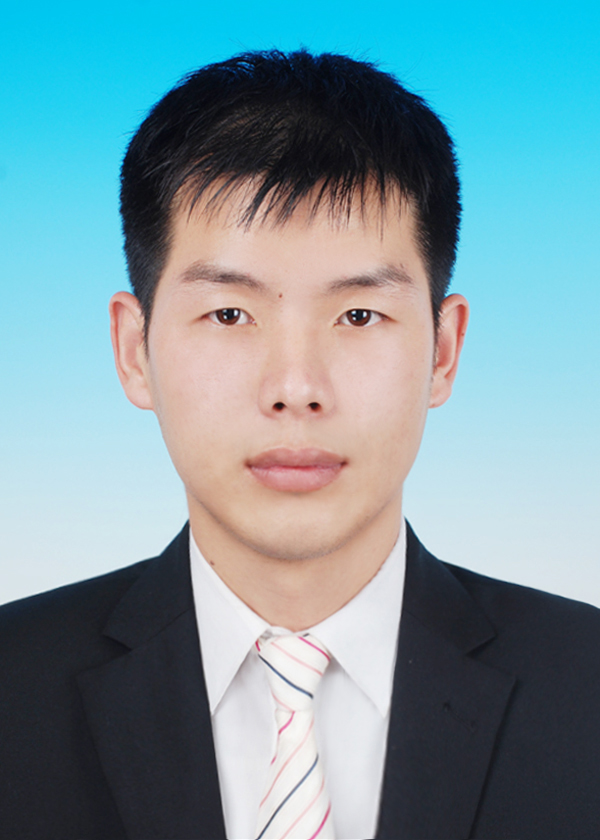
\includegraphics[scale=1.1]{8574.png}
\end{minipage}
\hfill
\begin{minipage}{0.8\textwidth}
	\renewcommand{\arraystretch}{2.2}
	\begin{adjustbox}{width=1\linewidth}
		\begin{tabular}{lcr}
			姓名: 张辉耀 & 性别:男 & 出生年月:1991.01.10 \\
			学历学位:博士研究生 & 政治面貌: 中共党员 & 婚否:未婚 \\
			邮箱: zhanghuiyao2357@163.com & 联系电话:152-1679-7320 & 户口所在地:河南驻马店 \\
			个人网站:\url{https://slip-slap.github.io/} & & 
		\end{tabular}
	\renewcommand{\arraystretch}{0.5}
	\end{adjustbox}
\end{minipage}




	\makecvfooter
	  {\today}
	  {HUIYAO ZHANG~~~·~~~CURRiCULUM ViTAE }
	  {\thepage}
	%-------------------------------------------------------------------------------
%	SECTION TITLE
%-------------------------------------------------------------------------------
\cvsection{}


%-------------------------------------------------------------------------------
%	CONTENT
%-------------------------------------------------------------------------------
\begin{cvparagraph}
研究生时期的导师为我打开了计算机世界的大门,从此以后,编程和数学从兴趣变成热爱。在过去六年的学术生涯中,
致力于研究先进的模型,算法在纺织服装,材料领域的应用和实践,并在计算机类的学术期刊上发表有两篇学术论文。使用的编程语言也从Matlab,到Java,到现在的python,C++。
为了方便学习和记录,把近些年的学习笔记放到个人GitHub网站上。未来主要想从事机器学习,数据科学以及人工智能方向的研究工作。
\end{cvparagraph}

	%-------------------------------------------------------------------------------
%	SECTION TITLE
%-------------------------------------------------------------------------------
\cvsection{Education}


%-------------------------------------------------------------------------------
%	CONTENT
%-------------------------------------------------------------------------------
\begin{cventries}

%---------------------------------------------------------
  \cventry
    {B.S. in Computer Science and Engineering} % Degree
    {POSTECH(Pohang University of Science and Technology)} % Institution
    {Pohang, S.Korea} % Location
    {Mar. 2010 - Aug. 2017} % Date(s)
    {
      \begin{cvitems} % Description(s) bullet points
        \item {Got a Chun Shin-Il Scholarship which is given to promising students in CSE Dept.}
      \end{cvitems}
    }

%---------------------------------------------------------
\end{cventries}

	%-------------------------------------------------------------------------------
%	SECTION TITLE
%-------------------------------------------------------------------------------
\cvsection{Research}

%-------------------------------------------------------------------------------
%	CONTENT
%-------------------------------------------------------------------------------
\begin{cventries}

%---------------------------------------------------------
  \cventry
    {Professor: Yokoyama Atsushi} % Advisor
    {Kyoto Institute of Technology} % Institution
    {Japan, Kyoto} % Location
    {2018.9 - now} % Date(s)
    {
      \begin{cvitems} % Description(s)
%		\item { The multiple constrained optimization based on a variant of
%				genetic algorithm(GA). GA is an efficient and robust algorithm
%				to solve the optimization problem in terms of discrete
%				variables.  However, intially GA was proposed for unconstrained
%				problem, to solve constrained problem, we have to reformulate
%				the objective function, in which append the constraints to the
%%				objective function as punishment items. To overcome the
 %   			inherient drawback, we propose a new genetic algorithm with two
 %   			techniques: mating pool classification and self-adaptive
 %   			mutaiton.  Then we adopt this new genetic algorithm to guide the
 %   			design of a laminate under single or multiple constraints.}
 %   			
 %%   	\item { The topology design of an artifical neural network(ANN) based on
  %  			genetic algorithm. Artifical neural networks are widely used for
  %  			various scenarios, such as prediction, classification,
  %  			optimization, in which the topology of an ANN plays a critical
  %  			role of the performance. We propose a three-layer ANN model, in
  %  			which the design variables are the number of neurons in the
  %%  			hidden layer, the active function, and the connection
   % 			relationship. Genetic algorithm is adopted to guide the search
   % 			process, and the one with best performance is used to predict
   % 			the strength of angle ply laminate. The advantage of the method
   % 			is to reduce the computaiton cost and simplify the
   % 			calculation process, compared with the tradional complicated
   % 			mathematical model.}
    %  \end{cvitems}
    }

%---------------------------------------------------------
  \cventry
    {Professor: Yueqi Zhong} % Advisor
    {Donghua University} % Institution
    {China, Shanghai} % Location
    {2015.9-2018.3} % Date(s)
    {
      \begin{cvitems} % Description(s)
        \item
			{
				The separation of connected curve based on convex hull algorithm
				and the elliptic curve fitting based on fourier transforamtion. 
				Convex hull algorithm is used to obtain the smallest convex
				polygon which encloses a set of points. Fourier transforamtion
				can be used to remove noises on a curve. The human body data
				points can be obtained through a three-dimensional scan device, 
				and the shape of transverse section of human body depends on the
				the cutting point. For the transverse section at the armpit, the
				shape of the cross section is a joint curve of three circles. We
				can use convex hull algorithm to find the separtion point. For
				the cross section at the waist, the corresponding shape is a
				circle with noises, and fourier transforamtion can remove the
				noise on the curve.
			}
      \end{cvitems}
    }

%---------------------------------------------------------
\end{cventries}

	%-------------------------------------------------------------------------------
%	SECTION TITLE
%-------------------------------------------------------------------------------
\cvsection{Publications}


%-------------------------------------------------------------------------------
%	CONTENT
%-------------------------------------------------------------------------------

%---------------------------------------------------------
%\cvsubsection{}
%---------------------------------------------------------


\begin{cvpubs}

%	\cvpub{
	\textbf{Huiyao Zhang}, Atsushi Yokoyama. 2022. Optimum Design of
	Laminated Composites for Minimum Thickness by a Variant of Genetic
Algorithm. Journal of Textile Engineering(accepted). 
%[收录: Scopus]
%}
	
%	\cvpub{
		\textbf{Huiyao Zhang}, Atsushi Yokoyama. 2021. A Technique for
		Constrained Optimization of Cross-ply Laminates Using a New Variant of
	Genetic Algorithm. International Journal of Advanced Computer Science and Applications, 12(6): 760-767. 
%[收录: Scopus/Web of Science(ESCI), 影响因子: 1.09]
%}

%	\cvpub{
		\textbf{Huiyao Zhang}, Atsushi Yokoyama. 2021. Predicting Strength
	Ratio of Laminated Composite Material with Evolutionary Artificial Neural
	Network. International Journal of Advanced Computer Science and Applications,
12(6): 11-18. 
%[收录: Scopus/Web of Science(ESCI),影响因子: 1.09]
%}

	%\cvpub{
		\textbf{Hui-Yao Zhang}, Duan Li, Hao-Yang Xie, Yue-Qi Zhong. 2017.
	A Study on the Female Chest Contour with Elliptic Fourier Analysis.
Journal of Fiber Bioengineering and Informatics, 10(3): 131-139.  %}

	%\cvpub{
		\textbf{Hui-Yao Zhang}, Duan Li, Hao-Yang Xie, Yue-Qi Zhong. 2017.
	Elliptic Fourier Analysis on Female Chest Contour. Textile Bioengineering
		and Informatics Symposium. 
%	[收录: CPCI(ISTP)/Scopus/Ei Compendex ]
	%}
\end{cvpubs}

% %---------------------------------------------------------
%\cvsubsection{In Review}
% %---------------------------------------------------------

%\begin{cvpubs}
%    \cvpub{Manuscript 1}

%    \cvpub{Manuscript 2}
%\end{cvpubs}

% %---------------------------------------------------------
%\cvsubsection{In Prep}
% %---------------------------------------------------------

%\begin{cvpubs}
%\small \color{black}
%    \cvpub{Manuscript 1}

%    \cvpub{Manuscript 2}
%\end{cvpubs}

% %---------------------------------------------------------

	%-------------------------------------------------------------------------------
%	SECTION TITLE
%-------------------------------------------------------------------------------
\cvsection{Presentation}


%-------------------------------------------------------------------------------
%	CONTENT
%-------------------------------------------------------------------------------
\begin{cventries}

%---------------------------------------------------------
  \cventry
    {Presenter for <Hosting Web Application for Free utilizing GitHub, Netlify and CloudFlare>} % Role
    {DevFest Seoul by Google Developer Group Korea} % Event
    {Seoul, S.Korea} % Location
    {Nov. 2017} % Date(s)
    {
      \begin{cvitems} % Description(s)
        \item {Introduced the history of web technology and the JAM stack which is for the modern web application development.}
        \item {Introduced how to freely host the web application with high performance utilizing global CDN services.}
      \end{cvitems}
    }

%---------------------------------------------------------
  \cventry
    {Presenter for <DEFCON 20th : The way to go to Las Vegas>} % Role
    {6th CodeEngn (Reverse Engineering Conference)} % Event
    {Seoul, S.Korea} % Location
    {Jul. 2012} % Date(s)
    {
      \begin{cvitems} % Description(s)
        \item {Introduced CTF(Capture the Flag) hacking competition and advanced techniques and strategy for CTF}
      \end{cvitems}
    }

%---------------------------------------------------------
  \cventry
    {Presenter for <Metasploit 101>} % Role
    {6th Hacking Camp - S.Korea} % Event
    {S.Korea} % Location
    {Sep. 2012} % Date(s)
    {
      \begin{cvitems} % Description(s)
        \item {Introduced basic procedure for penetration testing and how to use Metasploit}
      \end{cvitems}
    }

%---------------------------------------------------------
\end{cventries}

	%-------------------------------------------------------------------------------
%	SECTION TITLE
%-------------------------------------------------------------------------------
\cvsection{Skills}


%-------------------------------------------------------------------------------
%	CONTENT
%-------------------------------------------------------------------------------
\begin{cvskills}

%---------------------------------------------------------
  \cvskill
    {DevOps} % Category
    {AWS, Docker, Kubernetes, Rancher, Vagrant, Packer, Terraform, Jenkins, CircleCI} % Skills

%---------------------------------------------------------
  \cvskill
    {Back-end} % Category
    {Koa, Express, Django, REST API} % Skills

%---------------------------------------------------------
  \cvskill
    {Front-end} % Category
    {Hugo, Redux, React, HTML5, LESS, SASS} % Skills

%---------------------------------------------------------
  \cvskill
    {Programming} % Category
    {Node.js, Python, JAVA, OCaml, LaTeX} % Skills

%---------------------------------------------------------
  \cvskill
    {Languages} % Category
    {Korean, English, Japanese} % Skills

%---------------------------------------------------------
\end{cvskills}

	%-------------------------------------------------------------------------------
%	SECTION TITLE
%-------------------------------------------------------------------------------
\cvsection{Honors \& Awards}


%-------------------------------------------------------------------------------
%	SUBSECTION TITLE
%-------------------------------------------------------------------------------
\cvsubsection{International}


%-------------------------------------------------------------------------------
%	CONTENT
%-------------------------------------------------------------------------------
\begin{cvhonors}

%---------------------------------------------------------
  \cvhonor
    {Finalist} % Award
    {DEFCON 26th CTF Hacking Competition World Final} % Event
    {Las Vegas, U.S.A} % Location
    {2018} % Date(s)

%---------------------------------------------------------
  \cvhonor
    {Finalist} % Award
    {DEFCON 25th CTF Hacking Competition World Final} % Event
    {Las Vegas, U.S.A} % Location
    {2017} % Date(s)

%---------------------------------------------------------
  \cvhonor
    {Finalist} % Award
    {DEFCON 22nd CTF Hacking Competition World Final} % Event
    {Las Vegas, U.S.A} % Location
    {2014} % Date(s)

%---------------------------------------------------------
  \cvhonor
    {Finalist} % Award
    {DEFCON 21st CTF Hacking Competition World Final} % Event
    {Las Vegas, U.S.A} % Location
    {2013} % Date(s)

%---------------------------------------------------------
  \cvhonor
    {Finalist} % Award
    {DEFCON 19th CTF Hacking Competition World Final} % Event
    {Las Vegas, U.S.A} % Location
    {2011} % Date(s)

%---------------------------------------------------------
  \cvhonor
    {6th Place} % Award
    {SECUINSIDE Hacking Competition World Final} % Event
    {Seoul, S.Korea} % Location
    {2012} % Date(s)

%---------------------------------------------------------
\end{cvhonors}


%-------------------------------------------------------------------------------
%	SUBSECTION TITLE
%-------------------------------------------------------------------------------
\cvsubsection{Domestic}


%-------------------------------------------------------------------------------
%	CONTENT
%-------------------------------------------------------------------------------
\begin{cvhonors}

%---------------------------------------------------------
  \cvhonor
    {3rd Place} % Award
    {WITHCON Hacking Competition Final} % Event
    {Seoul, S.Korea} % Location
    {2015} % Date(s)

%---------------------------------------------------------
  \cvhonor
    {Silver Prize} % Award
    {KISA HDCON Hacking Competition Final} % Event
    {Seoul, S.Korea} % Location
    {2017} % Date(s)

%---------------------------------------------------------
  \cvhonor
    {Silver Prize} % Award
    {KISA HDCON Hacking Competition Final} % Event
    {Seoul, S.Korea} % Location
    {2013} % Date(s)

%---------------------------------------------------------
  \cvhonor
    {2nd Award} % Award
    {HUST Hacking Festival} % Event
    {S.Korea} % Location
    {2013} % Date(s)

%---------------------------------------------------------
  \cvhonor
    {3rd Award} % Award
    {HUST Hacking Festival} % Event
    {S.Korea} % Location
    {2010} % Date(s)

%---------------------------------------------------------
  \cvhonor
    {3rd Award} % Award
    {Holyshield 3rd Hacking Festival} % Event
    {S.Korea} % Location
    {2012} % Date(s)

%---------------------------------------------------------
  \cvhonor
    {2nd Award} % Award
    {Holyshield 3rd Hacking Festival} % Event
    {S.Korea} % Location
    {2011} % Date(s)

%---------------------------------------------------------
  \cvhonor
    {5th Place} % Award
    {PADOCON Hacking Competition Final} % Event
    {Seoul, S.Korea} % Location
    {2011} % Date(s)

%---------------------------------------------------------
\end{cvhonors}

}


%-------------------------------------------------------------------------------
\end{document}
